\documentclass[a4paper, 12pt]{report}
\usepackage[pdftex]{graphicx}
\usepackage[autostyle]{csquotes}
\usepackage[backend=bibtex,style=numeric,sorting=none]{biblatex}
\usepackage{caption}
\usepackage{subcaption} % for subfigure
\usepackage{hyperref}
\usepackage{amssymb}
\usepackage{tabularx}
\usepackage{multicol}
\usepackage{algpseudocode}
\usepackage{amsthm} % for theorem
\usepackage{algorithm}
\addbibresource{bibliography}

\theoremstyle{plain}
\newtheorem{thm}{Theorem}[chapter] % reset theorem numbering for each chapter

\theoremstyle{definition}
\newtheorem{defn}[thm]{Definition} % definition numbers are dependent on theorem numbers
\newtheorem{exmp}[thm]{Example} % same for example numbers

\begin{document}
\pagenumbering{roman}
\begin{titlepage}
\begin{center}

{\Huge \bfseries
Virtual Multi-Tenant Networks Simulator \\
using Software Defined Networks\\
}~\\[1cm]

% The '~' is needed because \\ only works if a paragraph has started.

{\large \bfseries
B.Tech. Project 1st Stage Report
}~\\[0.40cm]

{
Submitted in partial fulfilment of the requirements for the degree of
}~\\[0.20cm]

{\large \bfseries
Bachelor of Technology (Honors)
}\\[2.75cm]
\end{center}

\begin{multicols}{2}
\begin{flushleft}
{\large
\textit{Student:} \\
\textbf{Kausik Subramanian	} \\
\textbf{Roll No: 110050003}
}
\end{flushleft}
\columnbreak
\begin{flushright}
{\large
\textit{Guide:} \\
\textbf{Purushottam Kulkarni}
}
\end{flushright}
\end{multicols}

\vfill

\begin{center}

\includegraphics[width=4cm]{Figures/iitbblack.jpg}~\\[1cm]

{\large
Department of Computer Science and Engineering\\
Indian Institute of Technology Bombay\\
Mumbai 400076, India\\
}

\end{center}
\end{titlepage}
\chapter*{}
\begin{center}
\textbf{Abstract}
\end{center}
Abstract
\addcontentsline{toc}{chapter}{Abstract}
\begin{center}
{\large \bfseries
Acknowledgement
}~\\[1cm]
\end{center}
\begin{flushleft}
{
I wish to express my sincere gratitude and indebtedness to my guide, \\Purushottam Kulkarni and Umesh Bellur for their constant support and guidance throughout the project. I am also indebted to Martin Casado, whose talk on Software defined Networks at IIT Bombay inspired me to pursue research in the field. 
}~\\[1.5cm]
{
Kausik Subramanian\\
B.Tech. IV\\
CSE, IIT Bombay
}
\end{flushleft}

\tableofcontents
\pagenumbering{arabic}
\chapter{Introduction}

Introduction
\chapter{Problem Description}
With the advent of software-defined networks, data-centers allow \emph{tenants} its own network topology and control over the flow of its traffic. The mapping of virtual to physical topologies can be done with respect to various parameters, allowing efficient resource utilisation of the data-center. \\
Another use of network virtualization is that tenants can do a test-run of a network before deploying it in real life. Thus, a network testbed can be extremely useful. Developing a network testbed using SDNs due to its standard interface between controller applications and switch forwarding tables, which give great flexibility over the network. However, there is a lack of a physical SDN, thus we decided to use Mininet as the physical software defined network infrastructure to create virtual networks. With these motive, we developed \emph{POXVine}: POX Virtual Network Emulator (POX-VI-N-E).
POXVine takes input the topology specifications of the physical and virtual topologies, and produces a emulated network on Mininet. We describe the exact topology specifications in the next section.

\subsection{Topology Specification}
\subsubsection{Hosts}
For specifying the configuration of hosts, POXVine uses RAM size (in gigabytes) of host for deciding the placement of vrtual hosts on each host, i.e a virtual host with RAM size less than remaining capacity of a physical host can be placed on the host. We can safely disregard disk storage for VM placement (can use Network Storage).  We specify the IP address of the host in the configuration. The last field in the configuration is the switch this host is connected in the topology(physical or virtual). One assumption is that a host is only connected to a single switch in the network. 
\begin{verbatim}
	<server-name>  <RAM-size>  <ip-address>  <switch-name>
\end{verbatim}

\subsubsection{Switches}
POXVine uses Mininet to emulate OpenFlow-enabled switches. To simulate real network constraints, one of the important resources in software-defined networks is flow table size, especially in multi-tenant networks with thousands of hosts. Certain switches in the network can become a bottleneck due to excess of rules installed at the switch. 
\begin{verbatim}
<switch-name>  <flow-table-size>  
\end{verbatim}

\subsubsection{Links}
POXVIne uses Mininet to emulate the links connecting the hosts and switches. Each link is full-duplex (communication both ways) and the configuration specifies both the end-points of the link. Also, another important link parameter is \emph{bandwidth}. POXVine could be used to map virtual tenants providing \emph{minimum guarantees}. We can also have host mappings which try to minimise the bandwidth utilisation of the tenant. Since we are modeling small area networks (datacenters), we do not consider latency.
\begin{verbatim}
<entity-one-name>  <entity-two-name>  <link-bandwidth>  
\end{verbatim}

\subsection{Output}
The POXVine system takes the topology configurations as input, and provides a emulated virtual network mapped on the physical network using Mininet. POXVine preserves the \emph{virtual network abstraction} for each tenant network and also, we can analyse the physical network on which the virtual network is mapped.



\chapter{Related Work}
\begin{figure}
	\noindent
	\makebox[\textwidth]{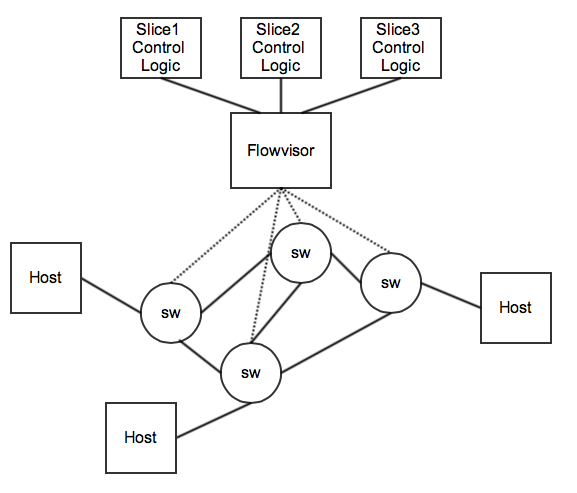
\includegraphics[width=12cm]{Figures/flowvisor.png}}%
	\caption{Flowvisor Architecture}
\end{figure}
One of our biggest motivations comes from Flowvisor \cite{flowvisor}, which slices the network hardware by placing a layer between the control plane and the data plane. Using  Flowvisor, we can split the network traffic into slices, and each slice can have its control logic. Using this, we can build a network testbed that is embedded in the physical network. \\
Flowvisor allows network researchers to test new protocols on production networks. It provides isolation between slices, so changes in one slice's control logic will not affect the other slices. Figure 3.1 illustrates the Flowvisor architecture. \\

Another work in this area is FlowN \cite{flown}, which deals with scalable Network Virtualization in software-defined networks. FlowN allows every tenant to run its own controller. The controllers are virtualized, so that the tenants' traffic are handled by the respective controller. For scalability purposes, FlowN uses databases to store the \emph{virtual-to-physical topology mappings}, thus capitalizing the years of research to achieve durable state and a highly scalable system.

\chapter{System Design}
POXVine consists of three main components.
\begin{itemize}
	\item The \emph{host mapper} is responsible to map the virtual network entities (hosts and switches) onto the physical topology. This mapping can be done based on different heuristics, so POXVine allows you to customize the host mapper. We have developed a host mapper \emph{MinSwitchMapper}, which tries to minimize the number of \emph{physical switches} which contain rules to the virtual topology.
	
	\item The \emph{network Mapper} is an application built over the \emph{POX} controller which uses the \emph{virtual-to-physical} mappings to add the required routing OpenFlow rules on the mininet switches, so that the virtual hosts can talk to one other. Another important design consideration is that the \emph{virtual network abstraction} must be preserved, that is, if a packet is to flow across a route in the virtual topology, on the physical topology, it must traverse the virtual network entities in the same order.
	
	\item The \emph{Mininet} infrastructure is used to emulate the physical network topology and the virtual hosts which are connected to the emulated physical switches (according to the \emph{virtual-to-physical}) mappings). 	
\end{itemize}  
I explain the individual components in the coming sections.


\begin{figure}
	\noindent
	\makebox[\textwidth]{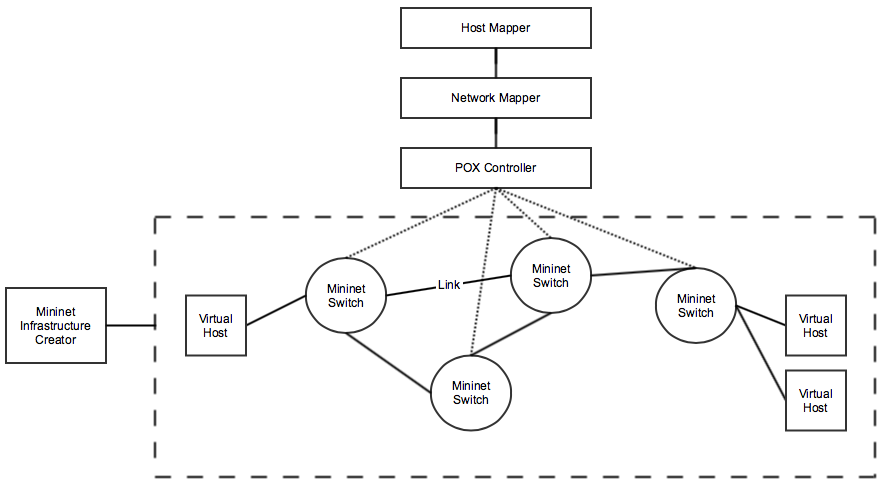
\includegraphics[width=17cm]{Figures/poxvine.png}}%
	\caption{POXVine Architecture}
\end{figure}

\section{MinSwitchMapper}
The host mapper module is responsible for finding the \emph{virtual-to-physical} mappings of the virtual network entities, i.e on which physical hosts, the virtual hosts and switches are placed. This mapping can be done according to various considerations, like \emph{maximizing number of virtual hosts, minimizing the number of switches mapped to a virtual topology, greedy host allocation, providing bandwidth guarantees etc.} \\
All the virtual network entities are mapped to physical hosts, which are connected by the physical network topology. Consider the network graph which is formed by using only the switches and links that are required to connect all the physical hosts (we use the shortest path between two hosts in the network graph). Figure 2.2 demonstrates an example of such a graph. 
\begin{figure}
	\noindent
	\makebox[\textwidth]{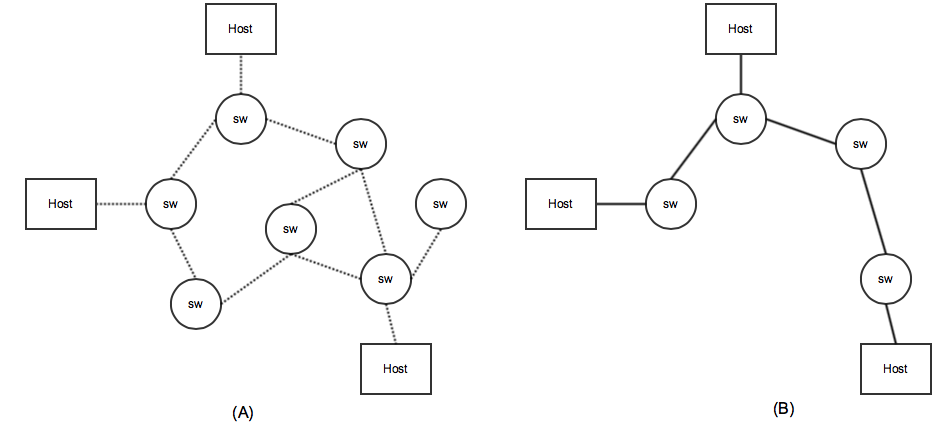
\includegraphics[width=17cm]{Figures/networkg.png}}%
	\caption{POXVine Architecture}
\end{figure}
\\
We have developed \emph{MinSwitchMapper}, which minimises the diameter of the network graph connecting the hosts of the virtual topology, The basis for this heuristic is that the traffic of this tenant's hosts are confined to the \emph{smallest portion} in the physical topology. This also minimises the number of switches where rules regarding this virtual topology is installed, thus increasing the number of tenants we can accomodate in POXVine (provided the physical host capacity is not insufficient)

\section{NetworkMapper}
The \emph{NetworkMapper} module is an application built on top of the POX controller. The role of the NetworkMapper is to use the \emph{virtual-to-physical mappings} generated by the host mapper module and add the required routing rules on the mininet switches for the virtual hosts of a tenant. One important design decision is that the NetworkMapper preserves the \emph{virtual network abstraction}. Let us suppose there are two virtual hosts \emph{v1} and \emph{v2}, connected by a path of two switches \emph{s1} and \emph{s2}, i.e $v1 \rightarrow s1 \rightarrow s2 \rightarrow v2 $.  Irrespective of the mapping, the Network Mapper must add the rules such that traffic from $v1 \rightarrow v2 $ must traverse through $s1$, $s2 $ and $v2$ in that order. 

\subsection{Route Tagging}




 


\chapter{Implementation}
\chapter{Evaluation}
\section{Correctness} 
For correctness, we create two virtual topologies : Vt1($h1,h2,h3$) and Vt2($h4,h5,h6$). Hosts in Vt1 and Vt2 must be able to talk to each other. And, since tenants are \emph{isolated} from each other, hosts of Vt1 should not be able to talk to Vt2 and vice-versa. The results of a \verb|pingall| operation in Mininet gives the following results, thus verifying correctness.
\begin{verbatim}
	> pingall
	h1 -> h2 h3 X X X
	h2 -> h1 h3 X X X
	h3 -> h1 h2 X X X
	h4 -> X X X h5 h6
	h5 -> X X X h4 h6
	h6 -> X X X h4 h5
\end{verbatim}
\section{Virtual Topology Mapping}
We create a \verb|TopologyCreator| class to create ring and tree topologies of custom length and depth respectively. To analyse the time complexity of mapping the virtual topology onto the physical topology, we create a tree topology of depth 10 as our physical topology and map virtual topologies of varying size and measure the time taken for the mapping. As we can observe in Figure 6.1 and 6.2, the time taken to calculate the mapping is constant across different virtual topologies(and less than 0.1 of a second). This follows from the algorithm as well, as the time complexity depends on the size of the physical topology.
\begin{figure}
	\noindent
	\makebox[\textwidth]{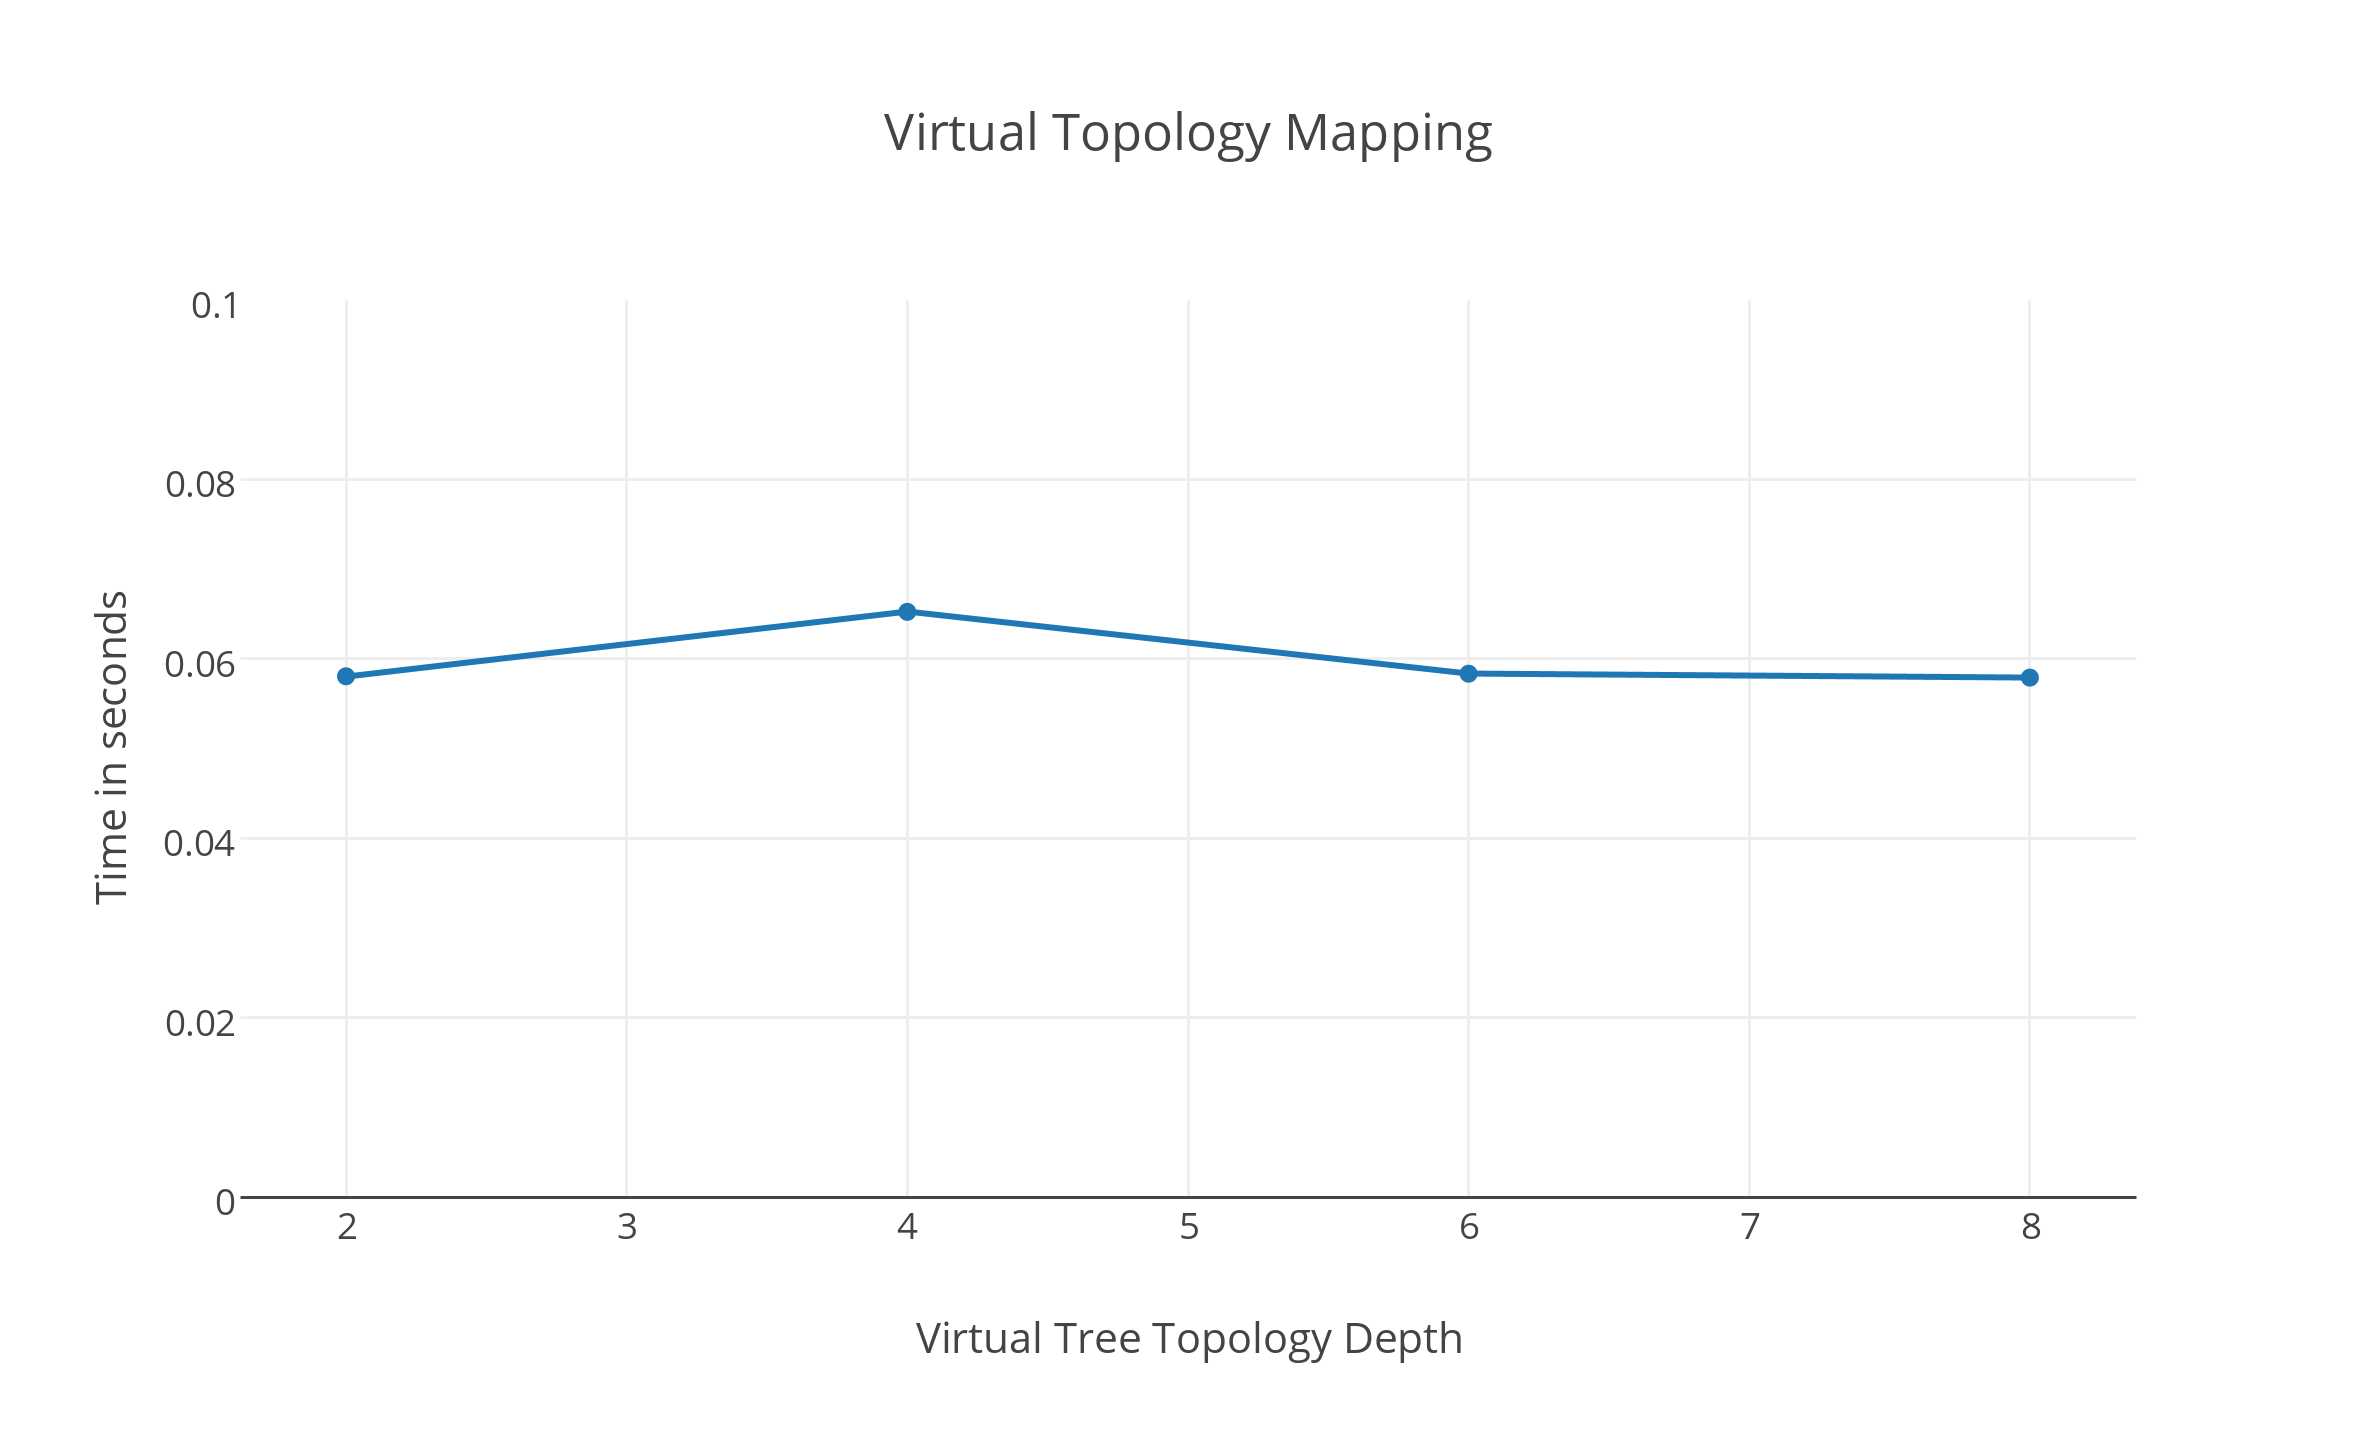
\includegraphics[width=15cm]{Figures/vtmt.png}}%
	\caption{Virtual Topology Mapping for varying tree topologies}
\end{figure}

\begin{figure}
	\noindent
	\makebox[\textwidth]{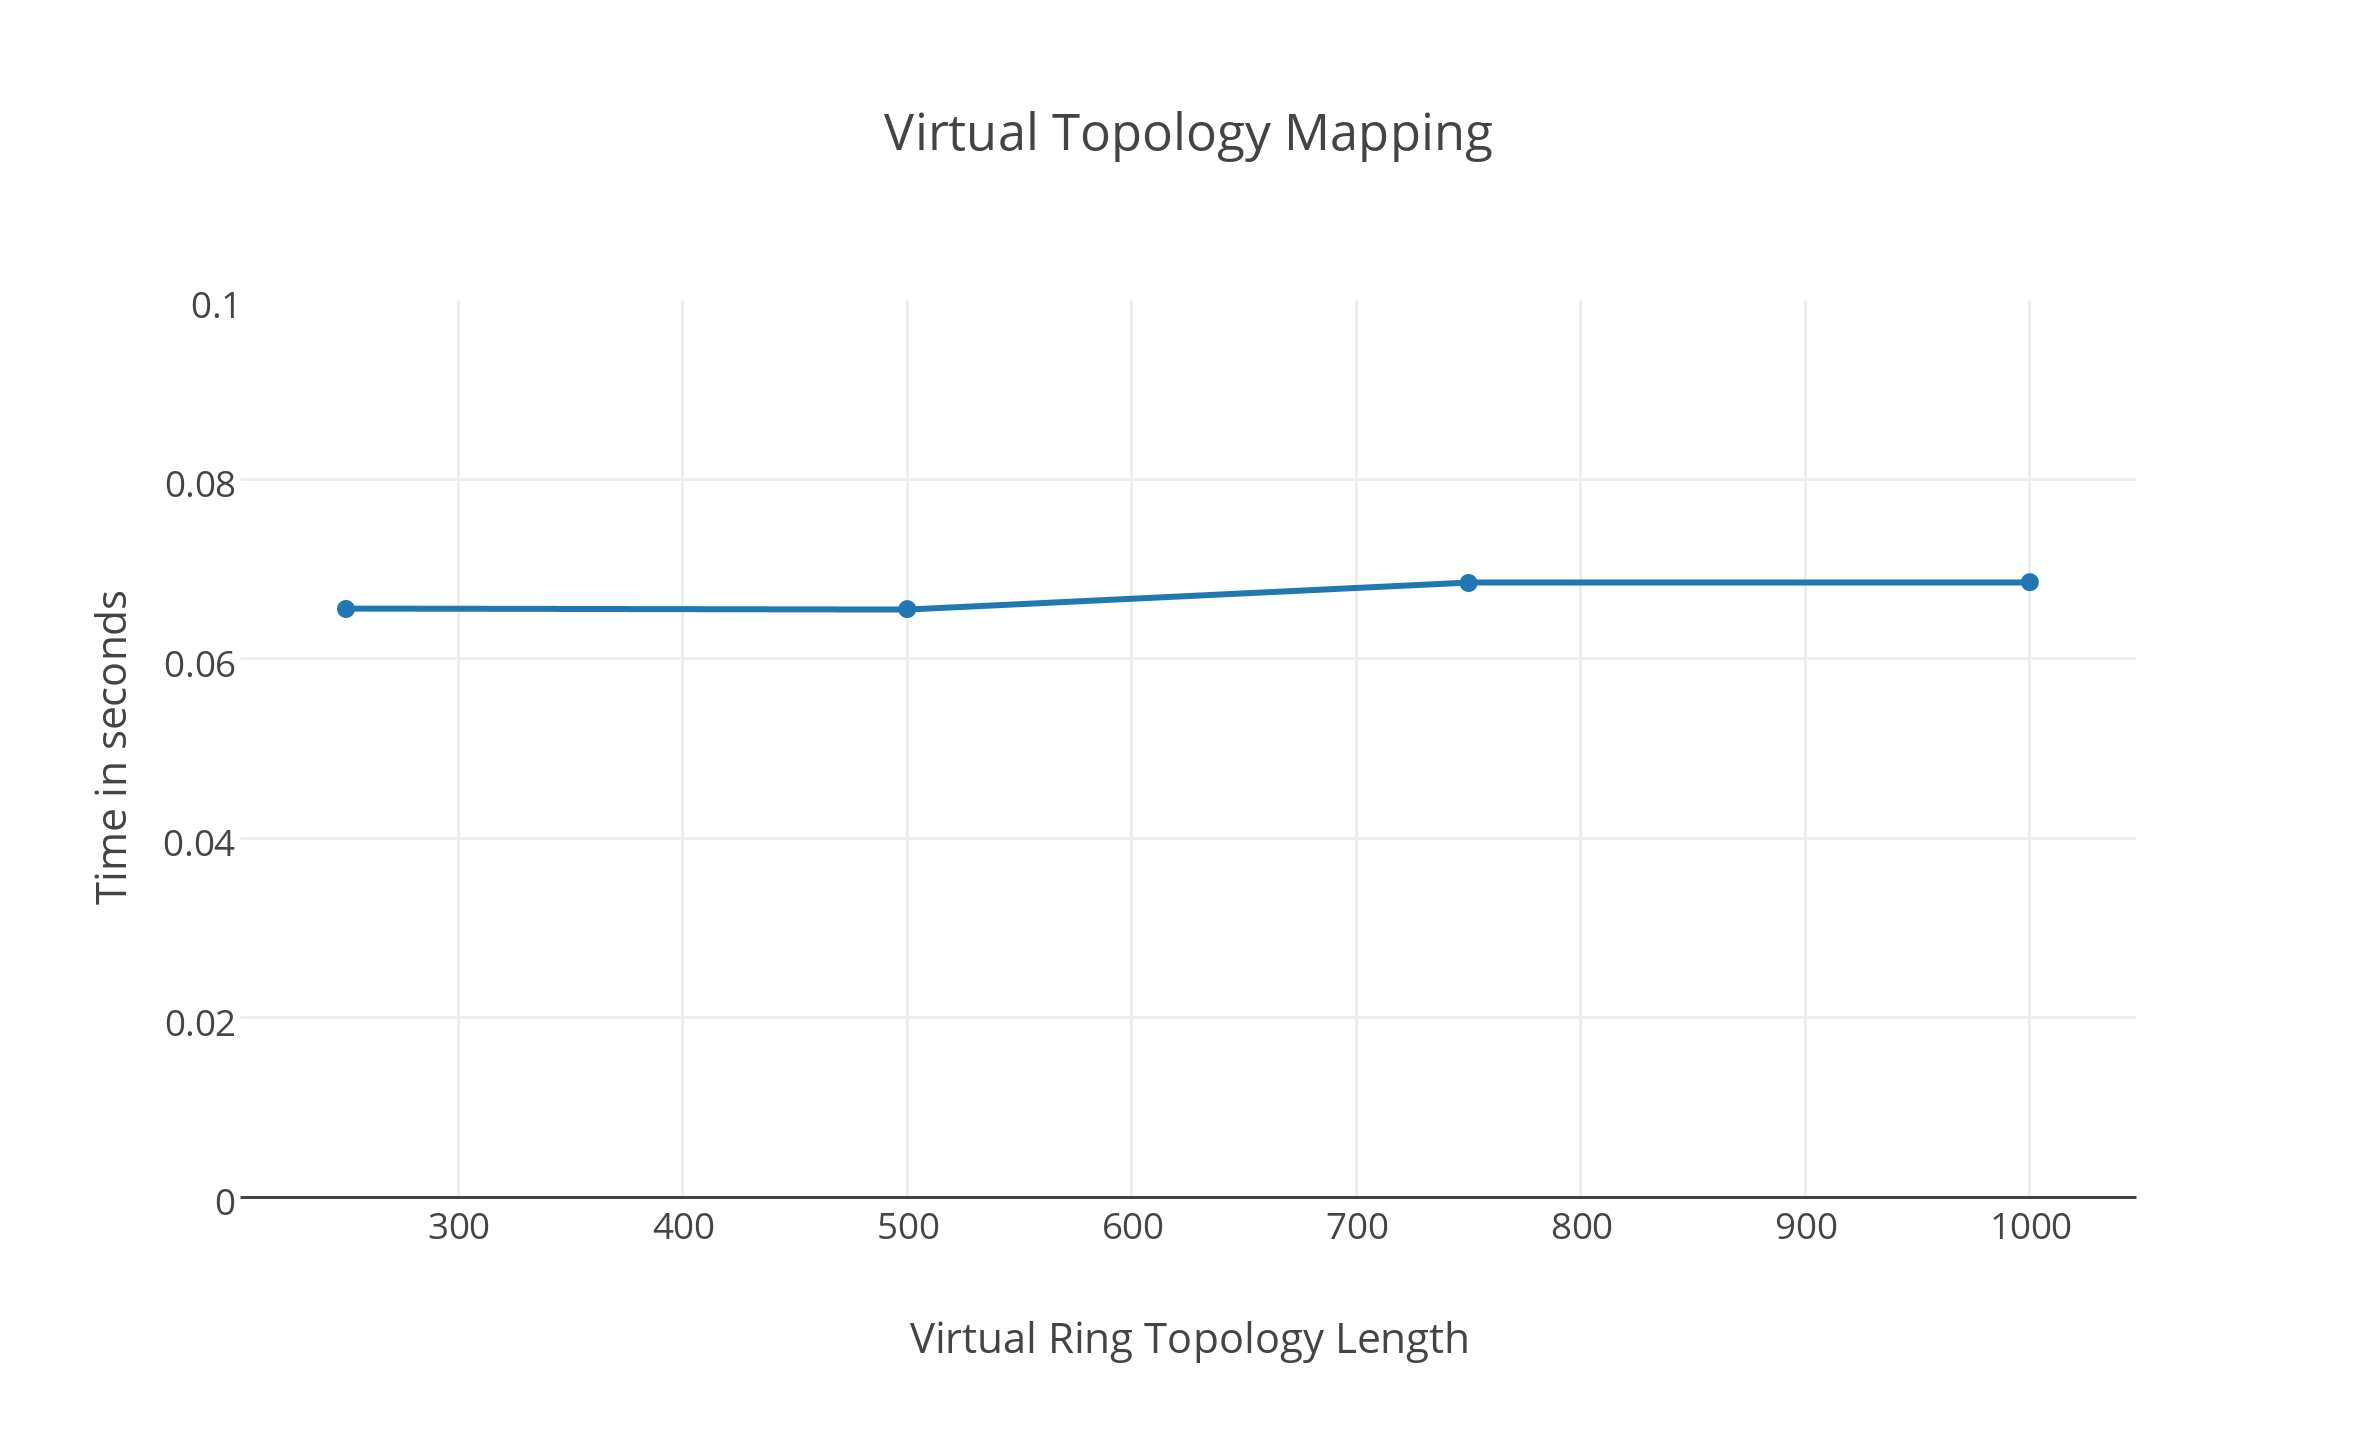
\includegraphics[width=15cm]{Figures/vmtr.png}}%
	\caption{Virtual Topology Mapping for varying ring topologies}
\end{figure}

\section{Network Route Calculation}
The next step is to calculate the \emph{complete} network routes between every pair of hosts in the virtual topology. We can infer that this time will be dependent on the sizes of both the virtual topology and physical topologies and the mapping heuristic used. Since we try to minimise the diameter of the mapped virtual network graph, we would obtain better results than other mapping schemes. The physical topology is a tree topology of depth 10 and we vary the mapped virtual topology sizes. Figures 6.3 and 6.4 plot the time taken to calculate the network routes for the varying virtual topologies. 

\begin{figure}
	\noindent
	\makebox[\textwidth]{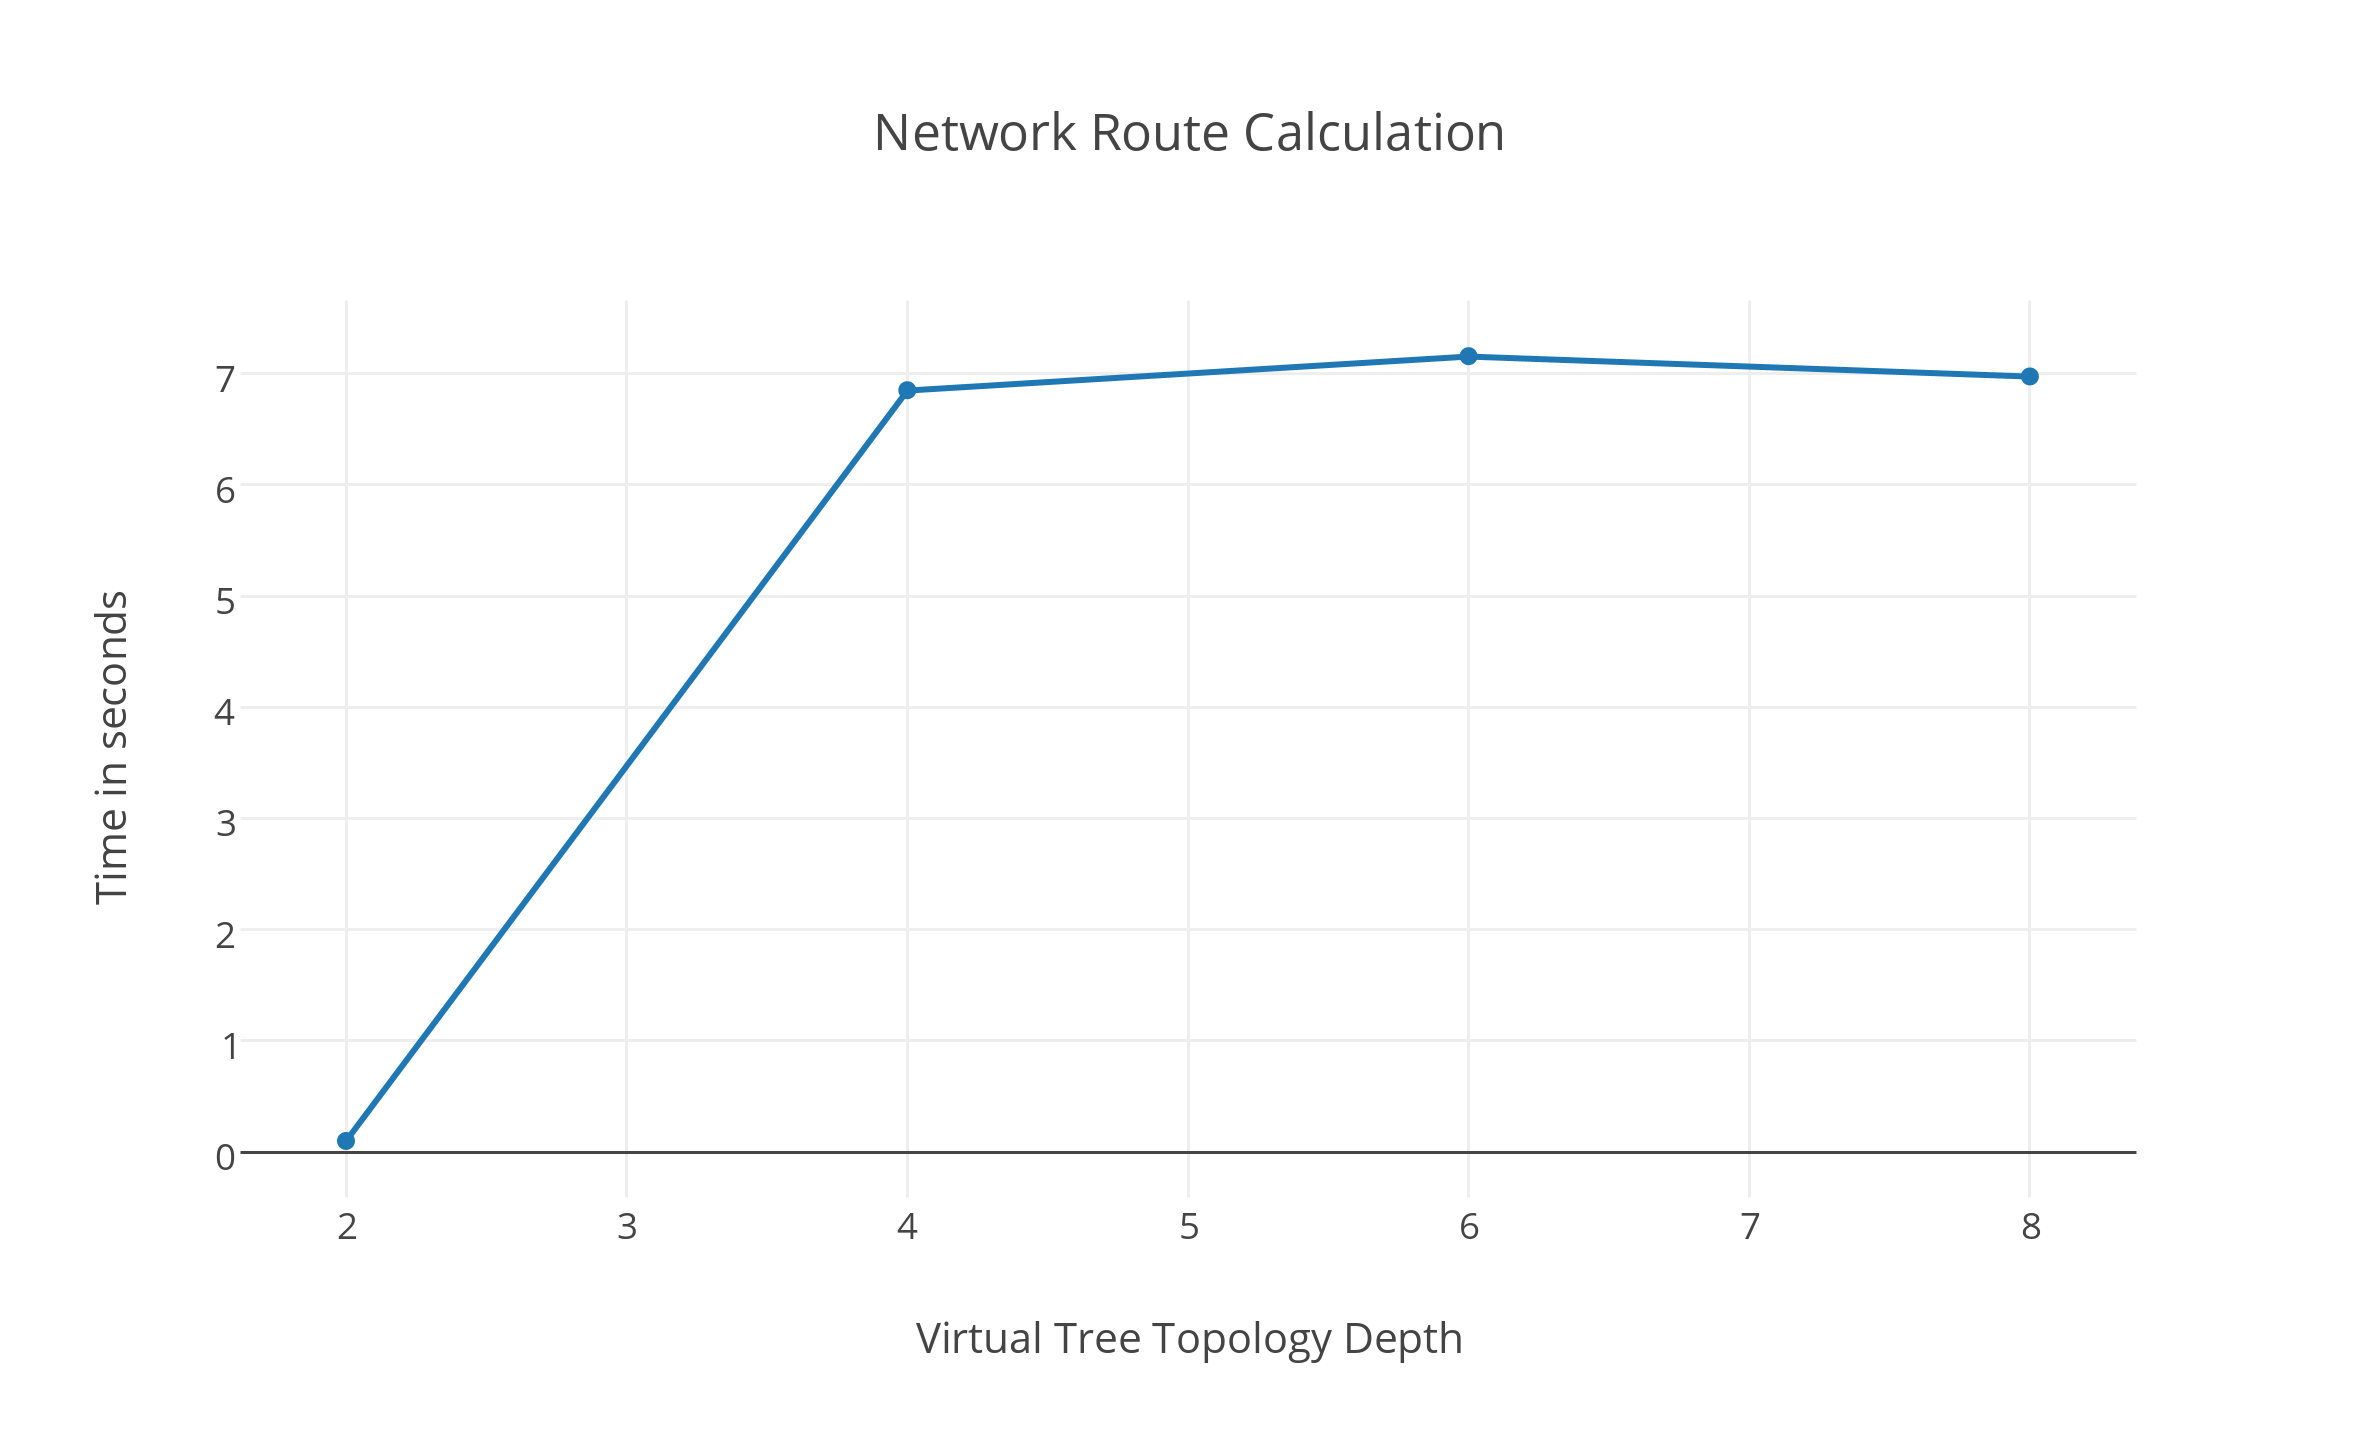
\includegraphics[width=15cm]{Figures/nrt.png}}%
	\caption{Network Route Calculation for varying tree topologies}
\end{figure}

\begin{figure}
	\noindent
	\makebox[\textwidth]{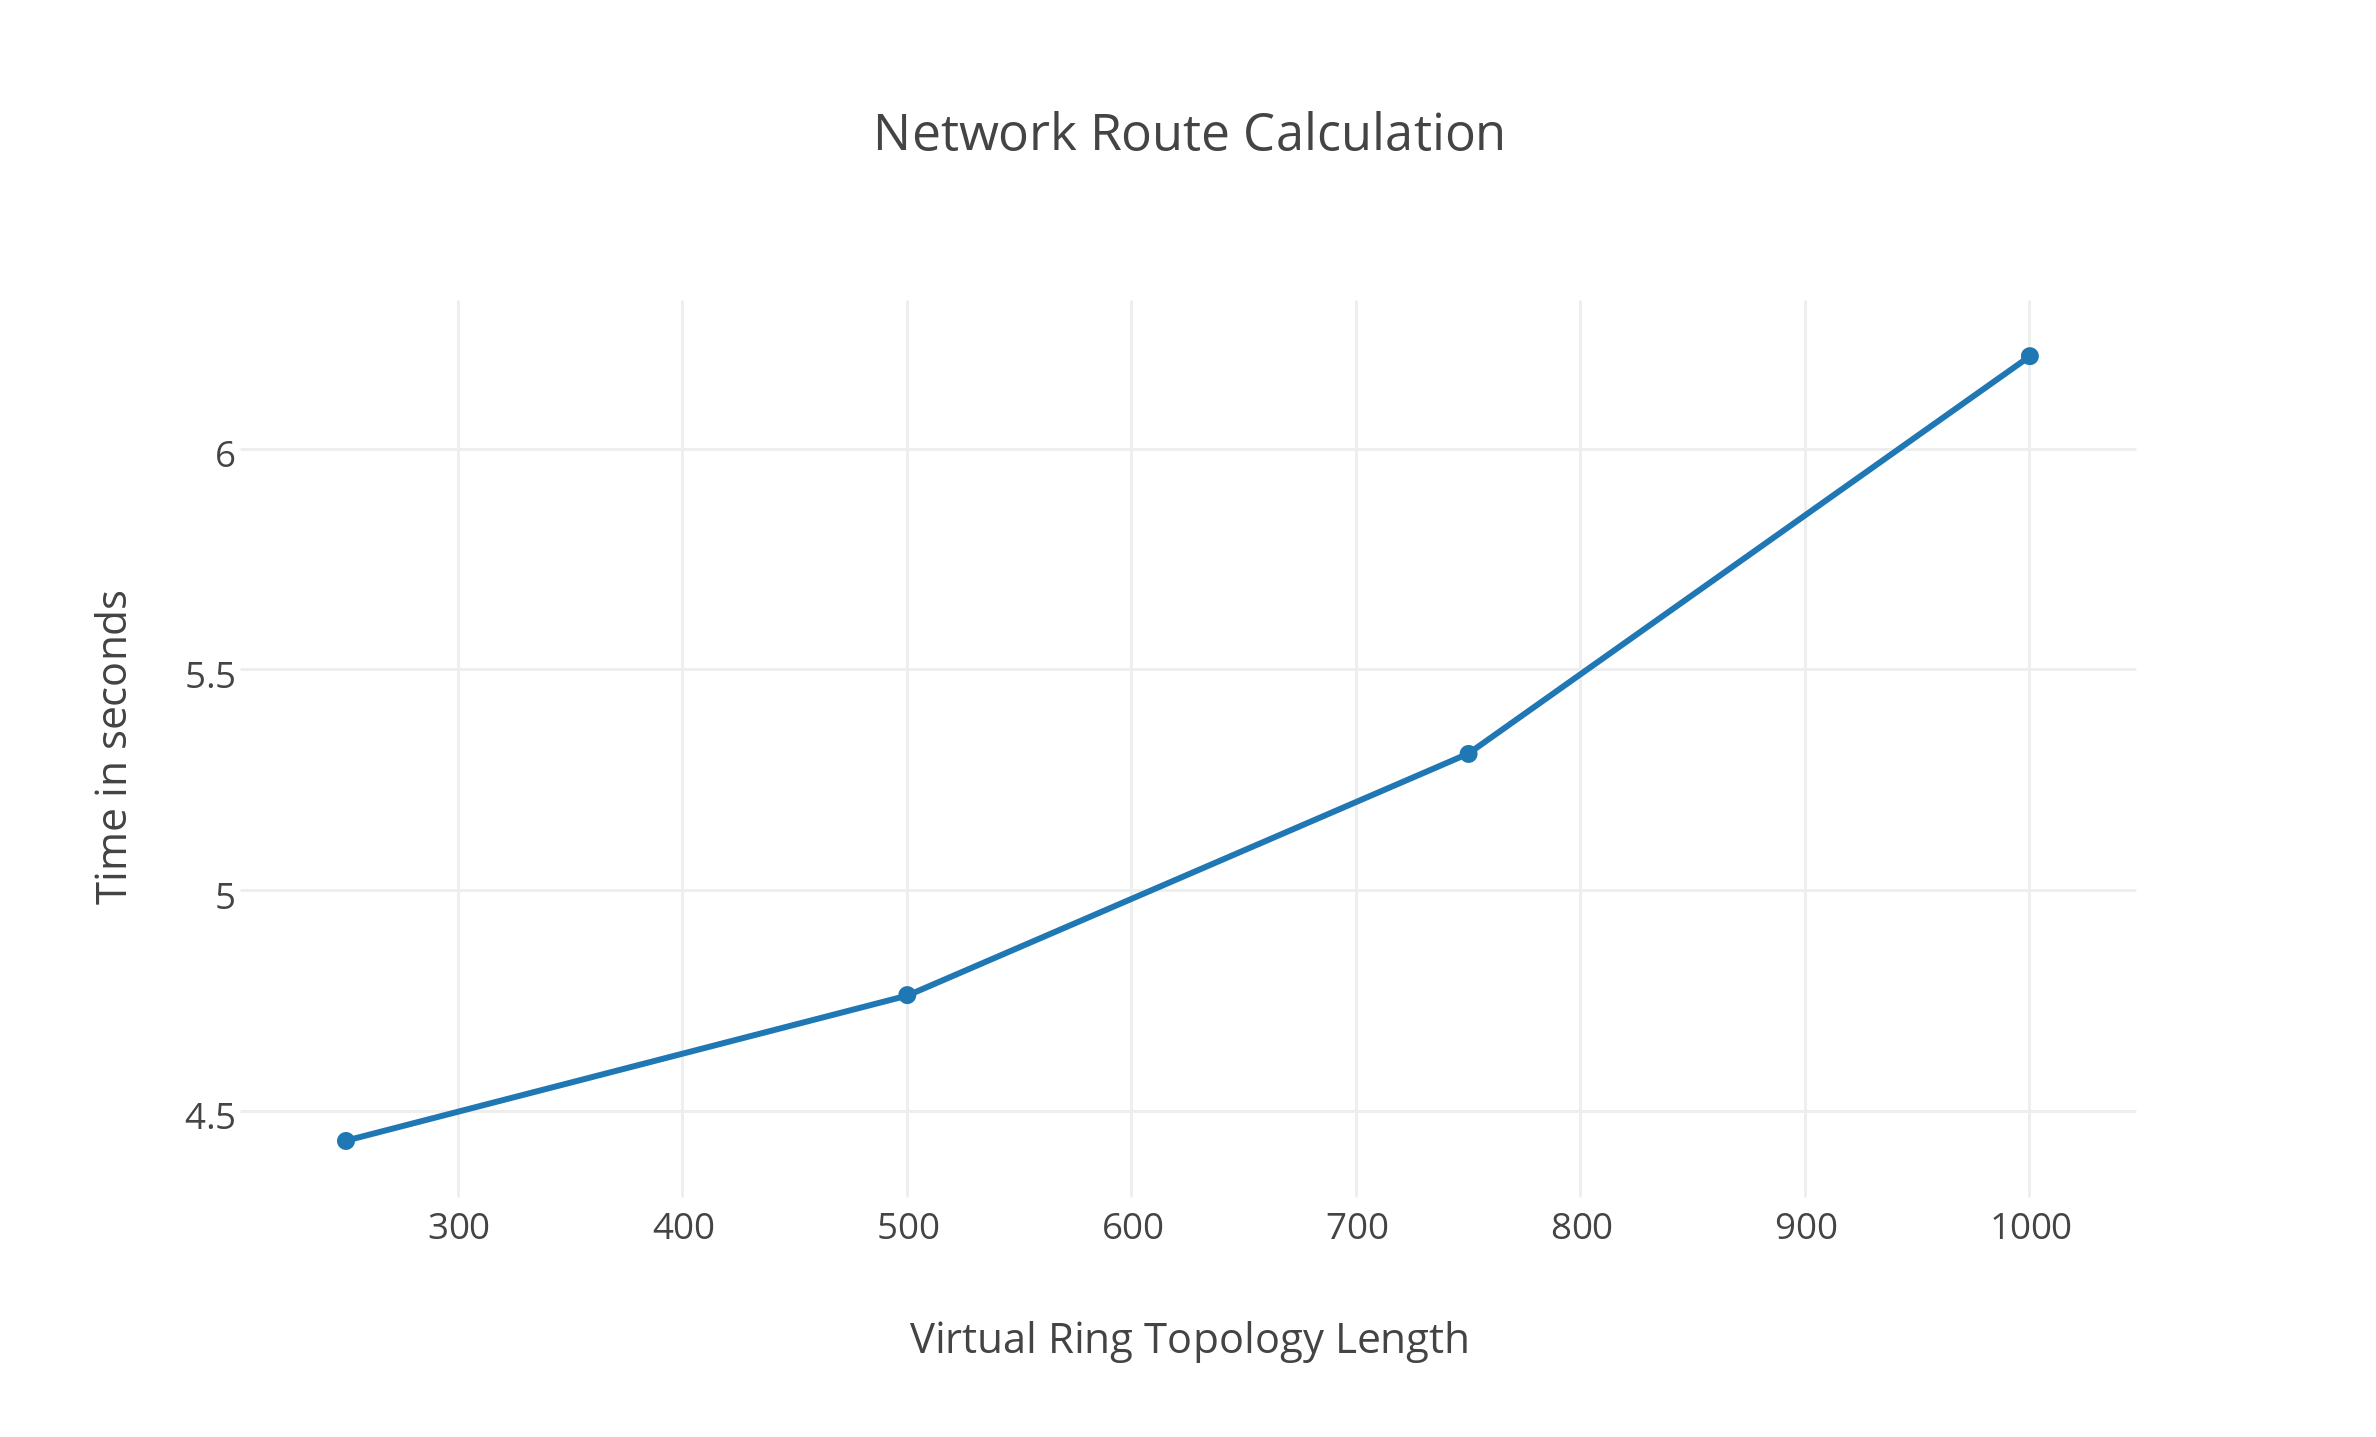
\includegraphics[width=15cm]{Figures/nrr.png}}%
	\caption{Network Route Calculation for varying ring topologies}
\end{figure}

\chapter{Future Work}
\begin{itemize}
	\item \emph{Providing minimum bandwidth guarantees to tenants}. One of the most important requirement for multi-tenant cloud services is providing certain bandwidth guarantees. We can analyse different bandwidth allocation schemes, and tenants can emulate the network and estimate their performance with respect to the provided bandwidth guarantees. Providing \emph{bandwidth guarantees}(\cite{secondnet}, \cite{oktopus}) is one of the hottest problems in the cloud. 
	
	\item \emph{ARP Packet Handling}. The ARP packets are not needed for communication between virtual hosts. For now, we have applied a \emph{ad-hoc} approach of flooding packets across the network, which will lead to wasteful congestion of the network. The approach is to build a ARP handler as a POX application which sends the \emph{ARP reply} to the \emph{ARP responses}. 
	
	\item \emph{Handling Link and Switch Failures} In real life networks, links and switches keep on failing. Thus, the NetworkMapper must be dynamic to these failures and calculate and install new forwarding rules to maintain the \emph{virtual network abstraction}.
	
	\item \emph{Running actual hosts and routers for virtual networks}. Presently, we emulate the virtual network using Mininet's hosts and Open VSwitches for routers. An extension is to be able to plug in software elements (like VMs and software routers)  to the Mininet backbone. This can help tenants test network configurations for correctness.  
	
	\item \emph{Network Testing as a  Cloud Service}. Many enterprises want to test out new networks before deployment for correctness, resource requirements, and so on. Developing POXVine as a cloud service can be extremely useful for enterprises who need not be concerned with operations related to network testing. Also, by designing a multi-tenant emulator, multiple tenants can share POXVine's resources, thus, we need not provision resources for each tenant (the benefit of cloud computing).
\end{itemize}


\chapter{Future Work}
Future Work

\pagenumbering{roman}
\printbibliography[heading=bibintoc]

\end{document}